\bf{Example}

Let $N=6,$ $M=6,$ $Q=3,$ $X=[5,1,1,3,3,5],$ $Y=[1,2,3,4,0,2],$ $S=[4,4,5],$ $E=[2,2,4],$ $L=[1,2,3],$ and $R=[2,2,4].$

The grader calls \t{check_validity(6, [5, 1, 1, 3, 3, 5], [1, 2, 3, 4, 0, 2], [4, 4, 5], [2, 2, 4], [1, 2, 3], [2, 2, 4]).}

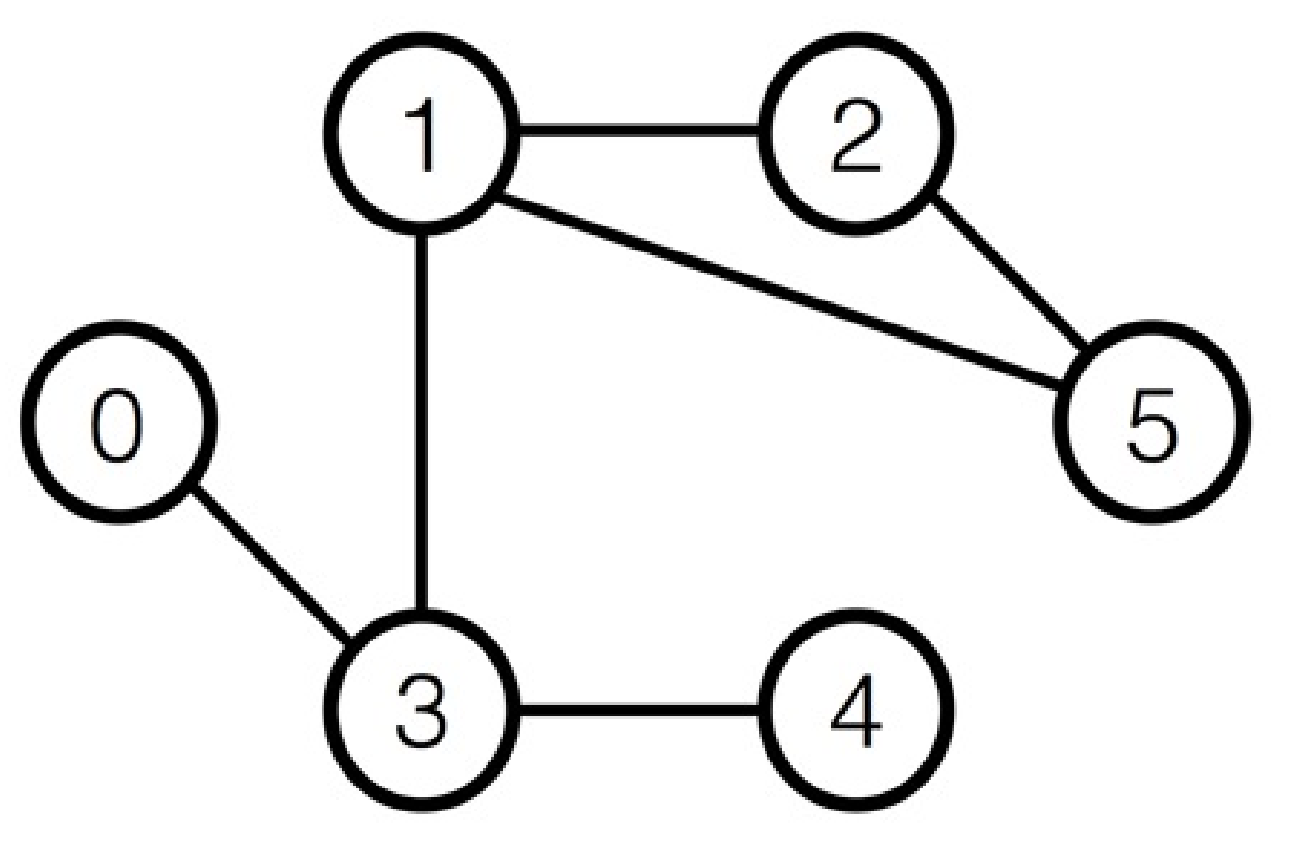
\includegraphics{image.png}

For the trip $0$, you can travel from the city $4$ to the city $2$ as follows:

\begin{itemize}
\item Start at the city $4$ (You are in human form) 
\item Move to the city $3$ (You are in human form)
\item Move to the city $1$(You are in human form) 
\item Transform yourself into wolf form (You are in wolf form) 
\item Move to the city $2$(You are in wolf form)
\end{itemize}

For the trips $1$ and $2$, you cannot travel between the given cities.

Hence, your program should return $[1,0,0].$

The files \t{sample-01-in.txt }and \t{sample-01-out.txt }in the zipped attachment package correspond to this example. This package also contains another pair of sample input/output files.
